% vim: textwidth=99 spell spelllang=en_gb:
% chktex-file 36

\documentclass[nobib, a4paper, twoside, justified]{tufte-book}

\usepackage[utf8]{inputenc}
\usepackage[british]{babel}
\usepackage{csquotes}
\usepackage[style=verbose, autocite=footnote, backend=biber]{biblatex}

\title{Displaying\\Heraldic\\Blazons}
\author{William Mathewson}
\publisher{University of Edinburgh}
\date{January 2018}

\addbibresource{bibliography.bib}

%%%%
%%
%% LOCALS are in `tufte-book-local.tex'

\usepackage{graphicx} % allow embedded images
\setkeys{Gin}{width=\linewidth,totalheight=\textheight,keepaspectratio}
\graphicspath{{graphics/}} % set of paths to search for images
\DeclareGraphicsExtensions{.pdf,.png}

\usepackage{amsmath}  % extended mathematics
\usepackage{booktabs} % book-quality tables
\usepackage{units}    % non-stacked fractions and better unit spacing
\usepackage{multicol} % multiple column layout facilities
\usepackage{fancyvrb} % extended verbatim environments
\usepackage{amsmath}
\usepackage{xspace}
\usepackage{makeidx}
\usepackage{mathtools}

\usepackage{float}
\usepackage{subfig}

\usepackage[final]{pdfpages}

%% Tell hyperref package it may break long URLs however it feels
\usepackage{hyperref}
\def\UrlBreaks{\do\/\do-}

%\newcommand{\dcim}{\emph{DCIM}\@\xspace}
%\newcommand{\ipam}{\emph{IPAM}\@\xspace}
%\newcommand{\dcimipam}{\emph{DCIM \& IPAM}\@\xspace}
%\newcommand{\desired}{\emph{desired}\@\xspace}
%\newcommand{\operational}{\emph{operational}\@\xspace}
%\newcommand{\wikid}{\textsc{WikiD}\@\xspace}
%\newcommand{\pywikid}{\textit{pywikid}\@\xspace}
\newcommand{\code}[1]{\texttt{#1}}
%\newcommand{\pythonthree}{Python$3$\@\xspace}

\newcommand{\svg}{\gls{svg}\@\xspace}
\newcommand{\svgs}{\glspl{svg}\@\xspace}
\newcommand{\dom}{\gls{dom}\@\xspace}

\newcommand{\charge}{\gls{charge}\@\xspace}
\newcommand{\charges}{\glspl{charge}\@\xspace}
\newcommand{\tincture}{\gls{tincture}\@\xspace}
\newcommand{\tinctures}{\glspl{tincture}\@\xspace}
\newcommand{\quarter}{\gls{quarter}\@\xspace}
\newcommand{\quarters}{\glspl{quarter}\@\xspace}

\newcommand{\blazon}{\gls{blazon}\@\xspace}
\newcommand{\blazons}{\glspl{blazon}\@\xspace}
\newcommand{\ublazon}{\Gls{blazon}\@\xspace}
\newcommand{\ublazons}{\Glspl{blazon}\@\xspace}

\newcommand{\payload}{\gls{payload}\@\xspace}
\newcommand{\payloads}{\glspl{payload}\@\xspace}

%\newcommand{\defeq}{\stackrel{\mathclap{\normalfont\mbox{def}}}{=}}
%\newcommand{\namedmap}[1]{\stackrel{\mathclap{\mbox{\small#1}}}{\longmapsto}}

%% R_{x->y} style
%\newcommand{\relate}[3]{\text{\itshape#1 }_{#2\ \mapsto\ #3}}

%% x --R--> y style
%\newcommand{\relate}[3]{#2\namedmap{#1}#3}

%% xRy style
%\newcommand{\relate}[3]{_{#2}#1_{#3}}

%\newcommand{\citetodo}{\sidenote{\todo{[Citation Needed]}}\@\xspace}
%\newcommand{\reftodo}{\sidenote{\todo{[Reference Needed]}}\@\xspace}
%\newcommand{\prooftodo}{\sidenote{\todo{[Substantiation Needed]}}\@\xspace}
\newcommand{\todo}[1]{{\noindent\textcolor{Red}{\textit{\quad#1}}\par}}

\let\lines\baselineskip{}

\usepackage[numberedsection=nameref]{glossaries}
\setacronymstyle{long-short}

\loadglsentries{glossary}

\glstoctrue{}

\begin{document}

\frontmatter

\maketitlepage{}

\abstract{In this project I describe how I designed and implemented a system to render heraldic
  blazons. Blazons are the text describing how shields in coats of arms are to be drawn. Through
  use of good software engineering principles, such as decoupling and delegation, I built a modular
  system that rendered the blazons with scope for further extension in the future. When comparing
against a similar system, it had significantly better performance with more features.}

\begin{publicationmeta}
  \section*{Acknowledgements}
  I would like to thank my supervisor, Julian Bradfield, for his help and advice as I was writing
  this project. I would also like to thank all my friends on Level 9 of Appleton Tower,
  particularly Connie, Nicole, Paul, Dan and Simon, who helped keep me going through the long,
  arduous journey that was this project and 4\textsuperscript{th} year as a whole.

  \section*{Declaration}
  I declare that this thesis was composed by myself,
  that the work contained herein is my own
  except where explicitly stated otherwise in the text,
  and that this work has not been submitted for any other degree or
  professional qualification except as specified.\par
  ({\textit{\thanklessauthor}})
\end{publicationmeta}

\tableofcontents

%\pagenumbering{Arabic}

\mainmatter%

\chapter{Introduction}%
\label{cha:introduction}

\section{Motivation}\label{sec:motivation}

In 1874 --- 4 years after his death --- John Papworth's \textit{Ordinary of British Armorials} was
published~\autocite{collins_1942}. In this work, he recorded approximately 50,000 descriptions of
families' coats of arms, none annotated.

This project makes it possible to have these descriptions, or \textit{\blazons} as they are termed
in heraldry (see~\ref{sec:heraldry}), drawn freely for people to view. This has potential
application for ancestry companies. Given the \blazon, they would be able to construct the shields
visually.

\section{Project Aim}%
\label{sec:project_aim}

This project was written as a paired project and as such, I only wrote the side of the project that
deals with rendering the \blazons, rather than the parsing. The parsing was implemented by my
partner, Anthony Gallagher, and, as such, this will not be covered in this report. Important shared
design elements will, however, be covered in Section~\ref{sec:core_concepts}.

The aim for this project was to design and implement a web app to render the parsed \blazon by
drawing \charges and \glspl{ordinary}.

\section{Contributions}%
\label{sec:contributions}

In this honours project, my contributions included:

\begin{itemize}
  \item Drawing the \charges and \quarters used on the shield, or \textit{\gls{escutcheon}},
  \item Writing the base web server and
  \item Writing the \quarter and \charge drawing algorithms.
\end{itemize}

\section{Report Structure}%
\label{sec:report_structure}

Following this chapter, the report is broken up into 5 further chapters with the following content:

\begin{itemize}
  \item \textbf{Chapter 2} presents the background surrounding the problem, with a beginner's
    guide to basic heraldry terms and the history surrounding heraldry, as well as other works
    related to this project;
  \item \textbf{Chapter 3} describes the overarching design decisions taken to guide the project in
    its implementation, along with its dependencies;
  \item \textbf{Chapter 4} provides an in-depth discussion of the iterative design and implementation
    process as I worked on solving the problem presented;
  \item \textbf{Chapter 5} evaluates the results, with regard to automated testing, other tools
    solving a similar, if not the same, problem, and shortcomings that the final implementation
    had; and
  \item \textbf{Chapter 6} concludes the work with further work that could be undertaken.
\end{itemize}

\chapter{Background}\label{cha:background}

\section{Heraldry}\label{sec:heraldry}

Many families, countries and organisations --- primarily in Europe --- have coats of arms. Coats of
arms were initially used on shields on the battlefield to identify individual knights, but later
came to be used as flags and banners for individuals and families of the upper classes at court.
The Royal Coat of Arms of the United Kingdom, belonging to the British monarch, can be seen in
Figure~\ref{fig:royal_coa}. If the reader wishes to learn more about heraldry and its history, I
would recommend the heraldic works of Charles Boutell and John Brooke-Little.

\begin{marginfigure}
  \centering
  \def\svgwidth{0.8\linewidth}
  \input{graphics/Royal_Coat_of_Arms_of_the_United_Kingdom.pdf_tex}
  \caption{The Royal Coat of Arms of the United Kingdom.
  Source:~\url{https://upload.wikimedia.org/wikipedia/commons/9/98/Royal_Coat_of_Arms_of_the_United_Kingdom.svg}}%
  \label{fig:royal_coa}
\end{marginfigure}

At the centre of a coat of arms is a shield known as an \textit{\gls{escutcheon}}. The language
used to describe how the escutcheon is to be drawn is known as a \textit{\blazon}.
\ublazons have been used since the Norman conquest and have been refined to a regular language
in the process~\autocite{boutell_1864}, although, as John Brooke-Little said, ``many of the
supposedly hard and fast rules laid down in heraldic manuals [including those by heralds] are often
ignored.''~\autocite{brooke_little_1985} This blatant disregard for the rules introduces
difficulty in parsing the \blazons as the language loses some of its regularity.

\begin{marginfigure}
  \centering
  \def\svgwidth{0.8\linewidth}
  \input{graphics/Blason_Albert.pdf_tex}
  \caption{The shield of the town of Albert, France. \textit{Barry of ten argent and
  gules}. Source:~\url{https://upload.wikimedia.org/wikipedia/commons/e/ee/Blason_Albert.svg}}%
  \label{fig:blason_albert}
\end{marginfigure}

\ublazons have 5 key attributes:
\begin{itemize}
  \item The \textit{\gls{field}}, which is the background colour of the shield or
    \quarter;
  \item \textit{\Glspl{ordinary}}, which are geometric shapes (as seen in Figure~\ref{fig:scrope},
    bearing a golden slash, or \textit{bend});
  \item \textit{\Glspl{charge}}, which are small emblems, such as fleur-de-lis and lions;
  \item \textit{\Glspl{variation}}, which describe how the field or \charge is patterned.
    \Glspl{variation} can indicate patterns such as chequered or coloured lines (as seen in
    Figure~\ref{fig:blason_albert}); and
  \item \textit{\Glspl{tincture}}, which are the colours and patterns for \charges, ordinaries
    and fields.
\end{itemize}

The tinctures are derived from Norman French and are divided into 3 groups, typically known as
\textit{metals}, \textit{colours} and \textit{furs}. In British heraldry, the colours are also
derived from Norman French and so the names appear archaic. In heraldry, blue is \textit{azure} and
red is \textit{gules} for instance. The metals are \textit{or} and \textit{argent}, for gold and
silver respectively. Whilst the tinctures are linked to colours, the College of Arms does not
specify which shade of that colour is required for the tinctures, leaving it to the artist to
decide~\autocite{college_of_arms_faq}. In this case, I have applied default CSS colours, using the
English names, for instance, `red' for \textit{gules}.

\begin{marginfigure}
  \centering
  \def\svgwidth{0.8\linewidth}
  \input{graphics/chief_example.pdf_tex}
  \caption{\textit{Purpure, a chief Gules}, as drawn by the project web app.}%
  \label{fig:chief_example}
\end{marginfigure}

\ublazons conventionally start with the \textit{\gls{tincture}} or \textit{\gls{variation}} of the
field. After the description of the field, \textit{\glspl{ordinary}} and \textit{\charges} are
named with their tinctures. An example of this is ``\textit{Purpure, a chief Gules}''. This \blazon
describes an escutcheon with a field of \textit{purpure} (purple), with a \textit{Chief}
\gls{ordinary} (a bar across the top of the shield) of \textit{gules} (red). This can be seen
 in Figure~\ref{fig:chief_example}.

\begin{marginfigure}
  \centering
  \def\svgwidth{0.8\linewidth}
  \input{graphics/scrope.pdf_tex}
  \caption{The Scrope \gls{escutcheon}; \textit{Azure, a bend Or}, as drawn by the project web app.}%
  \label{fig:scrope}
\end{marginfigure}

A simple, but notable, \blazon is that of the Scrope family. In the 14th century, the Baron Scrope
brought a case action against Sir Robert Grosvenor when he noticed that they both had the same coat
of arms. Many witnesses gave evidence in the case, including Geoffrey
Chaucer~\autocite{scrope_grosvenor}. The case was ultimately decided in Scrope's favour. The Scrope
coat of arms has a \blazon of \textit{Azure, a bend Or}; a depiction of this can be seen in
Figure~\ref{fig:scrope}.

Whilst the Scrope arms are prominent in heraldry, they are \\ simplistic and indicative of
medieval arms. Coats of arms became more complex as they developed through the centuries, with
instances of \textit{quarterly} shields, \textit{grand-quarterlies} --- quarterlies within
quarterlies --- and \textit{differenced} arms. \textit{Differenced} arms involve adding an
\gls{ordinary} over an existing coat of arms. This was typically used to differentiate similar
looking coats of arms, especially between father and sons. Common examples of differentiated
shields are seen in duchies' coats of arms, particularly those which were given to Charles II's
illegitimate children. Examples of more complex shields can be seen in
Figure~\ref{fig:complex_shields}.

\begin{marginfigure}
  \centering
  
\includegraphics[width=\linewidth]{of_the_first}
  \caption{\textit{Azure on a fess argent three billets azure} as rendered by \textit{pyBlazon}.
  See Section~\ref{sec:related_works}.}%
  \label{fig:of_the_first}
\end{marginfigure}

For a time, it was considered bad form to repeat a \textit{tincture} in a \blazon, and use a
reference to the tincture's previous use. The Heraldic Society gives an example as such:
``\textit{`Azure on a fess argent three billets azure'} [would have been written as] \textit{`Azure
on a fess argent three billets of the first'}''. The `\textit{of the first}' refers to the field's
tincture of azure. This \blazon describes a blue shield, with a white bar horizontally across the
middle with 3 white rectangles arranged along the bar. A rendering of this can be seen in
Figure~\ref{fig:of_the_first}. The Heraldic Society advocates repeating
tinctures to reduce ambiguity~\autocite{blazon_in_coa}.

\begin{figure}[h]
  \subfloat[Neville, 16th Earl of Warwick's coat of arms. An example of grand-quarterlies and
  differenced arms. Source:~\url{https://upload.wikimedia.org/wikipedia/commons/d/d1/Neville_Warwick_Arms.svg}.]{%
    \def\svgwidth{0.48\linewidth} %
    \input{graphics/Neville_Warwick_Arms.pdf_tex}
  }
  \qquad
  \subfloat[A quarterly shield drawn by the web app. \textit{Quarterly: 1st and 4th: Gules, a bend
  Sable; 2nd and 3rd: Azure, a chief Or}. ]{%
    \def\svgwidth{0.45\linewidth}
    \input{graphics/quarterly_example.pdf_tex}
  }
  \caption{2 examples of more complex coats of arms.}\label{fig:complex_shields}
\end{figure}

\section{Related Works}%
\label{sec:related_works}

Rendering \blazons has been partially implemented before: Robert Billard wrote
\textit{Blazons!}~\autocite{dos_blazon} for Windows 3.1 and 95 and Mark Shoulson and Arnt Richard
Johansen created \textit{pyBlazon}~\autocite{pyblazon} in 2008. \textit{Blazon!} does not parse a
blazon for automatic rendering, but provides an environment with predefined \charges and
\glspl{ordinary} to build one's own \glspl{escutcheon}. \textit{pyBlazon} solves this problem
exceptionally well, but does not render quarterly shields. Thus, a major goal of this project is to
support this. \textit{pyBlazon}, as the name suggests, is implemented in Python~\autocite{python}
and hosted in a PHP webserver. My intention to implement the rendering in
TypeScript~\autocite{typescript} (see Section~\ref{sec:core_concepts}) would aid portability, as
the code would be able to run on all modern browsers, whilst also being decoupled from the
back-end, allowing pluggable implementations of the parsing.

Despite the existence of these tools, they seem rarely used. Many escutcheons drawn and uploaded to
WikiMedia in \svg~\autocite{ferraiolo2000scalable} format appear to have been created in
Inkscape~\autocite{inkscape}. Much work has been done in collecting and cataloguing \blazons
themselves (especially John Papworth as mentioned in Section~\ref{sec:motivation}) giving plenty of
examples against which to test the finally completed application.

\section{Summary}%
\label{sec:background_summary}

In this chapter, we covered basic heraldry, including core terminology, as well as works related to
the project. Core heraldry terminology includes:

\pagebreak%

\begin{itemize}
  \item \textit{\Gls{escutcheon}} --- the shield in the coat of arms;
  \item \textit{\Gls{field}} --- the background of the escutcheon;
  \item \textit{\Glspl{ordinary}} --- geometric shapes on the escutcheon;
  \item \textit{\Glspl{charge}} --- small emblems, such as fleur-de-lis and lions; and
  \item \textit{\Gls{tincture}} --- the colours and patterns for \charges, ordinaries and fields.
\end{itemize}

All relevant heraldry terminology may be found in the Glossary on page~\pageref{main}.

\chapter{Design}%
\label{cha:design}

\section{Core Concepts}%
\label{sec:core_concepts}

The two languages chosen for implementing this project were Python~\autocite{python} and
TypeScript~\autocite{typescript}. Python was an optimal choice due to its good support for
\gls{nlp} through the \gls{nltk}~\autocite{bird2004nltk}. TypeScript is a typed superset of
JavaScript written by Microsoft that compiles to plain JavaScript. TypeScript was chosen as a more
expressive alternative to programming in pure JavaScript, thanks to the addition of powerful
features such as type assertions, access control and abstract classes. As a note to the reader, to
maintain interoperability with JavaScript, TypeScript adds type definitions after the variable
name, rather than before it, as in C. An example being that an \texttt{int} defined in C would be
`\texttt{int limit}', but in TypeScript, this would be `\texttt{limit:
number}'~\footnote{JavaScript/TypeScript uses a unified \texttt{number} type to handle both
\texttt{float}s and \texttt{int}s.}.

The core design for this project centres around having a split stack; with a Python back-end
parsing the \blazon, serialising it into JSON\footnote{\gls{json} is a lightweight data-interchange
  format, consisting of key-value pairs, array data types and other serialisable data types (such
  as strings, numbers and booleans). JSON is derived from JavaScript's associative array-style data
type, \texttt{Object}. An example of JSON can be seen in Figure~\ref{fig:expected_output}.} and
passing it to the TypeScript front-end, which would then draw it onto the webpage. This allows for
large amounts of flexibility, enabling the two halves of the project to be developed in tandem with
the Separation of Concerns principle being adhered to throughout. It also allows for pluggable
rendering implementations as the JSON for drawing \payloads can be specified.

The Python back-end receives a JSON \payload from the webpage containing the \blazon; it parses the
\blazon using a Context-Free Grammar (CFG) parser and identifies the most important parts of the
\blazon. It then serialises these back into a JSON response to be sent to the webpage for rendering.
The specification stated that if the webpage was given a \blazon of ``Azure, a bend Or'', it would
return the JSON response seen in Figure~\ref{fig:expected_output}.

\begin{figure}[h]
  \begin{verbatim}
    {
      "field": "azure",
      "charges": [{
        "charge": "bend",
        "tincture": "or"
      }]
    }
  \end{verbatim}
  \caption{Expected response from the Python back-end, for a given \blazon of ``Azure, a bend Or''.}%
  \label{fig:expected_output}
\end{figure}

\pagebreak%

The TypeScript front-end receives this response, applies the \texttt{azure} CSS class to the field
element, then draws a bend onto the field with an \texttt{or} CSS class. The rendering of this
response can be seen in Figure~\ref{fig:scrope}. The front-end does not use a framework and is
written in plain TypeScript.

Escutcheons are drawn using the \svg format for portability across browsers as well as the inherent
scalability of \svg images. This allows drawn escutcheons to be embedded elsewhere with ease,
either directly or through rendering the \svgs as other image formats via programs like Inkscape.

For version control, \texttt{git}~\autocite{git} was used and all code was hosted on GitHub.

\section{External Dependencies}%
\label{sec:external_dependencies}

The front-end depends on a pair of libraries for \svg rendering and \dom manipulation: the
selection library of D3.js~\autocite{d3js} and jQuery~\autocite{jquery}. D3.js and jQuery both
provide many powerful functions for \svg and \dom manipulation.  The \gls{w3c} \dom standard
defines the \dom as ``a platform and language-neutral interface that allows programs and scripts to
dynamically access and update the content, structure, and style of a document.'' The Mozilla
Developer Network adds to this, saying the \dom ``represents a document with a logical tree. Each
branch of the tree ends in a node, and each node contains objects.''~\autocite{mdn_dom}.

For further assets, Sass~\autocite{sass-lang} (a CSS extension language) was used as a CSS
pre-processor in combination with Bootswatch~\autocite{bootswatch-flatly} (a predefined CSS theme)
for the base styling. Webpack~\autocite{webpack} compiled TypeScript down to JavaScript ---
minifying and uglifying it in the process --- and concatenated all source files and their
dependencies into one main JavaScript file. \textit{\Gls{minification}} of JavaScript assets
involves stripping out all unnecessary whitespace and tokens.  \textit{\Gls{uglification}}
transforms the JavaScript code by renaming all variables and functions into short, obfuscated names
to reduce the footprint of the assets. These two techniques can decrease loading times of web apps
as the browser has to download smaller asset resources than the original, raw source code.

\subsection{Development Dependencies}%
\label{sub:development_dependencies}

To maintain code quality, TSLint~\autocite{tslint} (a TypeScript code linter) was set up to
automatically run as part of the Travis \gls{ci}~\autocite{travis} service, causing a build to fail
if the linter detected a style violation. For unit testing, Jest~\autocite{jest} (with
ts-jest~\autocite{ts-jest} for TypeScript support) was selected especially for its powerful mocking
and expectation matcher functionality. Automated documentation generation was provided by
TypeDoc~\autocite{typedoc}.

\section{Iterative Design}%
\label{sec:iterative_design}

An iterative design process was used for writing the code for this project. Iterative design is a
cyclical process of designing, prototyping and evaluating. In other words, one designs and
prototypes a new feature before evaluating the final feature design. If the design is acceptable,
the new feature is implemented, otherwise the cycle restarts. An iterative design process enables
one to address different functionality as separate tasks, building on top of one another. It also
allows for extensive refactors of a project whilst staying within one cycle.

\chapter{Implementation}%
\label{cha:implementation}

\section{Basic Charge Rendering}%
\label{sub:basic_charge_rendering}

\subsection{Design}%
\label{sub:first_design_iteration}

The first design iteration had a specific focus on basic \charge drawing.  The second iteration for
adding quarterly rendering, would rely on the results from this iteration.

I decided to have all drawing logic defined in the client, existing in a single module with minimum
dependencies. The shield outline was rendered on the page on load as part of the HTML template.
This supported a reliable entry point for the drawing logic as selecting the shield element was
straightforward. Having selected the element, the web app could begin appending other \svg elements
to it and enabled layering to be achieved. This is due to \svg ordering layers based on the order
of elements in the document. This was used to great effect when drawing quarters (see
Section~\ref{sub:second_design_iteration}).

The front-end was designed around functional paradigms; breaking up major functionality into
functions that would deal with smaller, encapsulated functionality, such as adding extra layers to
the HTML template or clearing the shield when drawing a new \blazon. This allowed for a stable API,
as the single point of access function would not be renamed, but all other functions may be changed
and updated separately. As described in Section~\ref{sec:core_concepts}, the front-end first
accessed the \texttt{field} value in the parsed JSON response, applied the value as the CSS class
for the shield and then moved onto the \charges. It iterated over the \texttt{\charges} array in
the JSON response, drawing each \charge onto the shield and applying the tincture as the CSS class.
Due to \svg layering, as mentioned earlier, if there were multiple \charges specified in the
response, all would be drawn according to the array ordering.

\subsection{Implementation}%
\label{sub:first_design_implementation}

As described in Section~\ref{sub:first_design_iteration}, the initial approach was to have all methods in
the core \texttt{index.ts} file that would be compiled and loaded in the browser. This
meant a smaller footprint when the code was bundled by Webpack and easier maintenance as all
relevant functions were next to one another, following the Step-Down
Rule~\autocite{martin2009clean}\footnote{The Step-Down Rule dictates that if function \texttt{A()}
calls function \texttt{B()} and \texttt{C()} in its function body, functions \texttt{B()} and
\texttt{C()} should be defined immediately after function \texttt{A()}.}.

\subsubsection{\texttt{drawShield(\blazon)}}%
\label{ssub:draw_shield}

The web app had a single entry point of \texttt{drawShield(\blazon)}, where \texttt{\blazon} was
the whole JSON response returned from the \texttt{/\_parse} endpoint on the web server (see
Figure~\ref{fig:expected_output} for an example JSON response). Initially this presented a problem
as TypeScript didn't handle the unstructured parsed data well due to it being a JavaScript
\texttt{Object}\footnote{In JavaScript, an \texttt{Object} works as both an associative array and a
basis for classes and inheritance through its \texttt{prototype} field.} instance. Attempting to
access members of this object (such as \texttt{\gls{field}}) caused TypeScript to produce an error
stating that the contents might be undefined and thus return a \texttt{null} object. To fix this, I
designed \texttt{interface}s with the expected fields in the \payload; one for the whole object,
\texttt{IBlazon}, and one for the \charges array contained within, \texttt{ICharge}. Similarly, to
avoid problems with string matching, I defined a pair of \texttt{enum}s to represent the supported
tinctures and \charges, \texttt{ETincture} and \texttt{ECharge} respectively. As discussed in
Section~\ref{sec:adding_quarterly_rendering}, I later added another \texttt{enum} for quarters.
All \texttt{interface}s and \texttt{enum}s can be found in Appendix~\ref{cha:interfaces_and_enums}.
Having fixed this data problem, \texttt{drawShield(\blazon)} was now able to access members of the
\blazon object safely.

\subsubsection{\texttt{clearShield()}}%
\label{ssub:clear_shield}

To avoid the problem of overlapping \charges, I had to write a \\ \texttt{clearShield()} method
that would iterate over all the \texttt{path} nodes in the \svg document, and delete them. This,
however, promptly deleted the shield outline, so I had to add a check to prevent deleting
\texttt{path} nodes with a \texttt{\#shield} id, instead only removing the CSS class. Having
cleared the shield of any possible obstructions, the \texttt{drawShield} method would then assign
the contents of the \texttt{field} value as the CSS class and iterate over the \texttt{\charges}
array, passing each \texttt{\charge} to \texttt{drawCharge(charge: ICharge)}.

\subsubsection{\texttt{drawCharge()} and \texttt{ChargeShapes}}%
\label{ssub:draw_charge}

When a \charge node is created in \texttt{drawCharge}, it is assigned an id. This id was formed
from the name of the charge, followed by a random number in the range $1\text{--}512$ inclusive.
This was later changed to rely on a cryptographically secure, random number generator, generating
unsigned 16-bit integers.

To draw shapes in \svg a \texttt{<path>} node requires a `\texttt{d}' attribute which contains the
commands for drawing that shape. To generate all these attributes, I drew all the \charge shapes in
Inkscape and extracted the `\texttt{d}' attributes from the generated \svgs. At first, I put a
\texttt{Map}\footnote{A \texttt{Map} here is a TypeScript/JavaScript data type, also known as a
\texttt{HashMap} or an associative array.} of the \charges and their paths in the global scope,
available for all functions to access. This worked for \charges that were produced using a
\texttt{path} node with a `\texttt{d}' attribute, but introduced a problem when using the chief
\charge (a chief \charge being displayed in Figure~\ref{fig:chief_example}). The chief \charge was
drawn using a \texttt{<rect>}\footnote{A \texttt{<rect>} node in \svg is used for drawing
rectangular shapes.} node which required `\texttt{x}' and `\texttt{y}' co-ordinates to specify a
starting point and \texttt{height} and \texttt{width} attributes to describe the size of the
rectangle. To address this, I wrote a \texttt{ChargeShapes} class to encapsulate the \charges and
their attributes. This class provided one public member, \texttt{chargePaths} which was of type
\texttt{Map<string, Map<string, string>\hphantom{}>}.  Representing this as a \texttt{Map} allowed
\texttt{drawCharge} to first check if the app knew how to draw the \charge by checking whether
\texttt{ChargeShapes.chargePaths} contained the \charge as a key.  If the \charge had an entry,
then \texttt{drawCharge} would iterate over the attribute \texttt{Map} and apply them to the
\texttt{<path>} or \texttt{<rect>} node, before finally applying the CSS class.

A visual representation of \texttt{drawCharge}'s execution may be seen in
Figure~\ref{fig:draw_charge}.

\begin{figure}
  \centering
  \subfloat[Initial \gls{escutcheon} outline on the webpage.]{%
    \def\svgwidth{0.45\linewidth}%
    \input{graphics/charge_renderer_process/draw_charge_stage0.pdf_tex}
  }
  \qquad
  \subfloat[First stage: applying the \texttt{field} CSS class.]{%
    \def\svgwidth{0.45\linewidth}%
    \input{graphics/charge_renderer_process/draw_charge_stage1.pdf_tex}
  }
  \\
  \subfloat[Second stage: drawing the charge onto shield.]{%
    \def\svgwidth{0.45\linewidth}%
    \input{graphics/charge_renderer_process/draw_charge_stage2.pdf_tex}
  }
  \qquad
  \subfloat[Final stage: applying the \texttt{tincture} CSS class on charge.]{%
    \def\svgwidth{0.45\linewidth}%
    \input{graphics/charge_renderer_process/draw_charge_stage3.pdf_tex}
  }
  \caption{The process of \texttt{drawCharge()} rendering a Scrope \gls{escutcheon}.}%
  \label{fig:draw_charge}
\end{figure}

The final part of \texttt{drawCharge} applied a transform to the \texttt{path} if the JSON response
included a boolean flag, \texttt{sinister}, to indicate that the bend \charge should be flipped.
This writes to an attribute \texttt{transform} which applies a \texttt{matrix} transformation that
flips the \charge followed by a \texttt{translate} transformation to move it into place. An
example of a sinister bend can be seen in Figure~\ref{fig:sinister_example}.

\begin{marginfigure}
  \centering
  \def\svgwidth{0.8\linewidth}
  \input{graphics/sinister_example.pdf_tex}
  \caption{\textit{Or, a bend sinister Vert.}}\label{fig:sinister_example}
\end{marginfigure}

\subsection{Evaluation}%
\label{sub:first_design_evaluation}

Whilst this simple implementation worked well for drawing basic \glspl{escutcheon}, like
Figure~\ref{fig:chief_example} and Figure~\ref{fig:sinister_example}, it wasn't able to draw more
complex shields like those seen in Figure~\ref{fig:complex_shields} and thus was not meeting the
project aims.

\section{Adding Quarterly Rendering}%
\label{sec:adding_quarterly_rendering}

\subsection{Design}%
\label{sub:second_design_iteration}

\subsubsection{Design Principles}%
\label{ssub:design_principles}

Whilst prototyping for adding functionality to render quarterly \\ shields, I found that it was
going to be impossible to maintain the initial, atomic design laid out in
Section~\ref{sub:first_design_iteration} whilst keeping the code clean and readable. This started
the second design iteration of the project. In this iteration, I designed a new, modular system
that leaned more heavily into Object-Oriented paradigms than functional ones. This new design was
written to enforce delegation and decoupling, whilst following the Single
Responsibility~\autocite{martin2000design} and Open/Closed principles~\autocite{martin2000design}.

The Single Responsibility principle dictates that a class should have one, and only one, reason to
change. If another responsibility is introduced, it should be given its own class. This principle
works well with decoupling as responsibilities can be changed in individual classes without
affecting other classes that depend upon it. The Open/Closed principle dictates that a class should
be open to extension but closed to modification. A typical example of this would be using abstract
classes; the interface specified by the abstract class is closed to modification, but the child
classes may extend the functionality in their implementation.

To comply with these principles, all major sections of functionality, including \blazon
\payload parsing, \charge and \quarter rendering, were encapsulated in their own classes with clear
names and well-defined, shared APIs.

\subsubsection{Top-Level Design}%
\label{ssub:top_level_design}

The new design had a top-level class of \texttt{\ublazon} which had a single public function,
\texttt{draw()}. The \texttt{draw} method, as before, would clear the shield and then delegate
drawing responsibility to specialised \texttt{\charge} and \texttt{\quarter} renderers by calling
their \texttt{draw()} methods. This \texttt{\ublazon} class became the new entry-point, being
instantiated and called in a \texttt{main()} function in \texttt{index.ts}. In a similar fashion to
the top-level \texttt{\ublazon} class, a \texttt{\Gls{quarter}} class was defined to enable proper
delegation for rendering both the \quarter \textit{and} the \charges contained within the quarter.
The new \texttt{ChargeRenderer} class would contain most major logic for drawing, as well as
\texttt{id} generation. \texttt{QuarterRenderer} extended \texttt{ChargeRenderer} to add
\quarter-specific logic, while also being able to call up to it to draw the contained \charges.

For a quarterly \blazon, the \payload would have the \texttt{\gls{field}} value set to
\texttt{``quarterly''} and rather then having a field \texttt{charges: ICharge[]}, it would contain
a field \texttt{quarters: IBlazon[]}. This worked as \quarters are treated as their own small
\glspl{escutcheon} in heraldry and are described as such. An example of a quarterly \blazon would
be \textit{Quarterly: 1st and 4th: Gules, a bend Sable; 2nd and 3rd: Azure, a chief Or}, as seen in
Figure~\ref{fig:complex_shields}. The expected JSON response for this \blazon can be seen in
Figure~\ref{fig:quarterly_json_output}. It was then possible to change functionality of the app
depending on the contents of the \texttt{field} key. To account for the new quarters that needed to
be drawn, a new \texttt{enum} \texttt{EQuarter} was designed, with the members being the positions
of the \svg elements and the \texttt{path}s in the \texttt{ChargeShapes.chargePaths} \texttt{Map}.

\subsubsection{Applying \svg Properties}%
\label{ssub:using_svg_for_great_good}

In this refactor, I also made use of more \svg properties: clip paths and the \texttt{<g>} element.
Clip paths allowed defining a path that cropped the element it was defined on. This was
particularly useful for drawing \charges inside of \quarters as the edges outside of the \quarter
would be cropped out by the clip path defined for that \quarter. The \texttt{<g>} element is a
grouping element for \svg; it applies all transformations defined on it to all of its child
elements and any of its attributes are also inherited. I used the \texttt{<g>} elements for both
grouping together charges and quarters, and explicitly named layers for the shield outline and the
\charges within.

\begin{figure}[h!]
  \begin{verbatim}
  {
    "field": "quarterly",
    "quarters": [
      {
        "field": "gules",
        "charges": [
          {
            "charge": "bend",
            "tincture": "sable"
          }
        ]
      },
      {
        "field": "azure",
        "charges": [
          {
            "charge": "chief",
            "tincture": "or"
          }
        ]
      },
      {
        "field": "azure",
        "charges": [
          {
            "charge": "chief",
            "tincture": "or"
          }
        ]
      },
      {
        "field": "gules",
        "charges": [
          {
            "charge": "bend",
            "tincture": "sable"
          }
        ]
      }
    ]
  }
  \end{verbatim}
  \caption{Expected JSON response from the Python back-end for a given \blazon of
  \textit{Quarterly: 1st and 4th: Gules, a bend Sable; 2nd and 3rd: Azure, a chief Or}.}%
  \label{fig:quarterly_json_output}
\end{figure}

\pagebreak%

\subsection{Implementation}%
\label{sub:nd_design_implementation}

%The Figure references in the following headings refer to the UML diagrams in
%Appendix~\ref{sec:second_design_iteration_diagrams}.
%UML diagrams for all classes mentioned in this subsection can be found in
%Appendix~\ref{sec:second_design_iteration_diagrams}.

\subsubsection{\texttt{\ublazon}}%
\label{ssub:blazon}

\texttt{\ublazon} took two arguments in its \texttt{constructor}: \texttt{svg} and \texttt{data}.
\texttt{svg} was a D3.js~\autocite{d3js} data type that contained a selector for the \texttt{<svg>}
element in the HTML document, for appending elements to. This data type is henceforth referred to
as \texttt{d3.Selection}. The \texttt{data} argument took the full JSON response returned by the
parser. The \texttt{constructor} would then turn the \texttt{data} \texttt{Object} into a
\texttt{Map} object for more reliable access. To get more fine-grained access to the \svg document,
the \texttt{constructor} populated extra fields by selecting the whole shield element and the
\texttt{<g id=``charge\_layers''>} element, these being defined within the \texttt{svg} selection.
The \texttt{chargesLayer} field is required for telling the renderer classes where to draw their
shapes.  Depending on the contents of the JSON response, the \texttt{constructor} would then
instantiate either new \texttt{ChargeRenderer} objects, or 4 new \texttt{Quarter} objects.

\texttt{clearShield} was extracted from \texttt{index.ts} into \texttt{Blazon}, but with changes to
account for the many \texttt{<path>} nodes as well as \texttt{<clipPath>} elements. The method
iterated over child elements of the \\ \texttt{<g id=``charge\_layers''>}, which were \texttt{<g>},
\texttt{<path>} and \texttt{<rect>} nodes, and \texttt{<clipPaths>} with an \texttt{id} beginning
with \texttt{``quarterly\_''}, deleting them in the process. It also stripped the \texttt{shield}
node of its CSS class.

A UML diagram for \texttt{\ublazon} may be seen in Figure~\ref{fig:BlazonUML} in
Appendix~\ref{sec:second_design_iteration_diagrams}.

\subsubsection{\texttt{Quarter}}%
\label{ssub:quarter}

The new \texttt{Quarter} class relied on the order of the \texttt{quarters} array in the response
to determine which quarter it was representing; with numbering starting at 0 in the top left
quarter, going left to right, ending at 3 in the bottom right. The ordering of the
\texttt{quarters} array may be seen in Figure~\ref{fig:quarterly_json_output}. The
\texttt{constructor} required the array index as its first argument, with \texttt{field:
ETincture}, \texttt{charges: ICharge[]}, \texttt{svg} and \texttt{chargesLayer} as its other
arguments. With these parameters, the \texttt{constructor} selected the quarter specified by the
\texttt{index}, instantiated \texttt{ChargeRenderer} objects --- borrowing a method from
\texttt{Blazon} --- and a \texttt{QuarterRenderer} object. The \texttt{draw()} method of
\texttt{Quarter} first called the \texttt{draw()} method on the \texttt{QuarterRenderer} object to
draw the quarter \texttt{path} onto the shield, then called \\ \texttt{addClipPathDefinition(svg)}
(see~\nameref{ssub:charge_renderer}) to add a new clip path to the \svg document. Having used
\texttt{QuarterRenderer} to draw a new quarter \texttt{path}, it selected it, assigned it to a
locally scoped constant, \texttt{quarterLayer}, and iterated over the \texttt{charges}. Before
calling the \texttt{draw} method on the \texttt{charge} object, it called the \\
\texttt{updateChargesLayer} on the \texttt{charge} object, passing it the \\ \texttt{quarterLayer}
to instruct the \charge to render in the \quarter.

A UML diagram for \texttt{Quarter} may be seen in Figure~\ref{fig:QuarterUML} in
Appendix~\ref{sec:second_design_iteration_diagrams}.

\subsubsection{\texttt{ChargeRenderer}}%
\label{ssub:charge_renderer}

The \texttt{constructor} for \texttt{ChargeRenderer} expected a \texttt{chargesLayer}, a
\texttt{tincture: ETincture}, a \texttt{charge: ECharge | EQuarter} and a \\ \texttt{sinister:
boolean} argument. The \texttt{tincture} argument was used by both the \texttt{ChargeRenderer}
itself and the \texttt{QuarterRenderer}, for the colour of the \charge and \gls{field}
respectively. The union type signature of \texttt{charge} allowed it to draw both \charges and
\quarters, as appropriate. For the drawing logic itself, I extracted the \texttt{drawCharge}
function from the \texttt{index.ts} file into the \texttt{ChargeRenderer} \texttt{draw()} method.
However, in trying to keep extensibility from \texttt{ChargeRenderer} to \texttt{QuarterRenderer},
the logic was then extracted from the \texttt{draw} method into its own protected
\texttt{drawCharge(}\texttt{currentCharge: d3.Selection,} \texttt{chargeLayer?: d3.Selection)}
method. This freed up the \texttt{draw} \\ method to handle setting up the \svg document for the
\quarters and \charges to be drawn into, as well as applying clip paths.

Whilst implementing \charge rendering within \quarters, I found that I needed to change the
layer that \charges were being drawn in to. I decided to add a new method to allow updating
the \texttt{chargesLayer} after a \texttt{ChargeRenderer} object had been instantiated.

The \texttt{getRandomInt} method was also extracted from the \texttt{index.ts} file
into \texttt{ChargeRenderer} for \texttt{id} generation.

\subsubsection{\texttt{QuarterRenderer}}%
\label{ssub:quarter_renderer}

\texttt{QuarterRenderer} extended \texttt{ChargeRenderer}, with few changes to \\ what it
inherited. Rather than generating a random \texttt{id} for the quarter, it used the \texttt{charge:
ECharge | EQuarter} parameter (that would be a member of \texttt{EQuarter} in this case). A new
method \\ \texttt{addClipPathDefinition(svg)} was also added. In \svg documents, clip paths are
defined using \texttt{<clipPath>} elements inside a \texttt{<defs>} element at the top of the
document. The \texttt{addClipPathDefinition} method selected the \texttt{<defs>} element and
appended a \texttt{<clipPath>} element, before updating the \texttt{chargesLayer} and calling the
inherited \texttt{drawCharge} method.

A UML diagram for \texttt{ChargeRenderer} and \texttt{QuarterRenderer} may be seen in
Figure~\ref{fig:charge_renderer_hierarchy} in Appendix~\ref{sec:second_design_iteration_diagrams}.

\subsection{Evaluation}%
\label{sub:second_design_evaluation}

This design iteration had brought quarterly rendering a lot closer to fruition, as seen in
Figure~\ref{fig:second_iteration_progress}, however proper scaling and translation of charges was
yet to be implemented. The project aims were yet to be realised. When adding the
functionality to apply quarter-specific transformations, I had difficulties maintaining clean,
extensible code. To both satisfy the project aims and the code standards, I had to redesign how
\texttt{ChargeShapes} and both \texttt{Renderer} classes worked.

\begin{figure}
  \centering
  \subfloat[The expected output for the blazon \textit{Quarterly: 1st and 4th: Gules, a bend
  Sable; 2nd and 3rd: Azure, a chief Or}.]{%
    \def\svgwidth{0.4\linewidth}
    \input{graphics/quarterly_example.pdf_tex}%
  }
  \qquad
  \subfloat[The second iteration output of this blazon.]{%
    \def\svgwidth{0.4\linewidth}%
    \input{graphics/second_iteration_quarterly.pdf_tex}
  }
  \caption{Second iteration progress.}%
  \label{fig:second_iteration_progress}
\end{figure}

\section{Refactoring Charge Rendering}%
\label{sec:refactoring_charge_rendering}

\subsection{Design}%
\label{sub:third_design_iteration}

\subsubsection{\texttt{Renderer} Hierarchy}%
\label{ssub:renderer_hierarchy}

This new design made use of the \textit{Liskov Substitution} and Open/Closed
principles~\autocite{martin2000design}. The Liskov Substitution principle dictates that derived
classes must be substitutable for their base class. Abstract classes are a good application for
this principle as they provide a reliable interface and force inheriting classes to implement the
abstracted methods defined within. As a reminder, the Open/Closed principle dictates that classes
should be closed to modification but open to extension.

Applying these principles, I redesigned the rendering structure to have common methods and
attributes belonging to both \\ \texttt{ChargeRenderer} and \texttt{QuarterRenderer} in a new
abstract parent class, \texttt{Renderer}. This refined and enforced the previously specified API of
render classes having a main entry-point of \texttt{draw()}. Using an abstract class gave
assurances to classes that used its implementations that there would always be a \texttt{draw()}
function. It also gave child classes the shared functions that both required, whilst allowing them
to specialise in their individual use cases. This enabled previously ambiguous attributes to be
renamed more specifically for their particular \texttt{Renderer} implementation. An example is
where \texttt{ChargeRenderer} previously had \texttt{charge:~ECharge~|~EQuarter}, it \\ now had
\texttt{charge:~ECharge}.

The planned execution for this design may be seen in Figure~\ref{fig:quarter_rendering}.

\subsubsection{\texttt{ChargeShapes} and \texttt{QuarterShapes} Abstraction}%
\label{ssub:chargeshape_and_quartershape_abstraction}

In a similar fashion to the \texttt{Renderer} redesign, I devised a new design for the attributes
and transforms for \texttt{ChargeShapes}. Rather than having all paths defined in a \texttt{Map} on
\texttt{ChargeShapes}, a new abstract class, \texttt{AShape}, would be defined with a
\texttt{dimensions} \texttt{Map} and a \\ \texttt{transforms(transform: string): string} method.
Each charge then extended \texttt{AShape}, implemented the two abstract properties and was imported
by the \texttt{ChargeShapes} class. The \texttt{ChargeShapes} class was redesigned to have a
boolean function, \texttt{hasChargePath(charge:\\ string)}, to check if it knew the given charge.
\texttt{ChargeShapes} also had a static function, \texttt{chargeShapes(charge: ECharge)}, which
returned an instance of \texttt{AShape}. This design makes use of the \textit{Dependency Inversion}
principle~\autocite{martin2000design}, which says that a class should depend on abstractions,
rather than concretions. In this case, when renderers call out to \texttt{ChargeShapes} for the
relevant \texttt{chargeShapes} object, they are returned an \texttt{AShape} object. This increases
reusability as well as extensibility of charge rendering, as one just needs to create a new
\texttt{AShape} class, import it into the \texttt{ChargeShapes} class and add it to the relevant
methods.

Quarter shapes were also extracted into their own hierarchy, mirroring that of the \texttt{AShape}
hierarchy. \texttt{AQuarterShape} only exposed a \texttt{dimensions} \texttt{Map} however.

%Dependency Inversion - \texttt{AShape}, \texttt{AQuarterShape}

\begin{figure}
  \centering
  \subfloat[Initial \gls{escutcheon} outline on the webpage.]{%
    \def\svgwidth{0.425\linewidth}%
    \input{graphics/quarter_renderer_process/stage0.pdf_tex}
  }
  \qquad
  \subfloat[Drawing on the quarter shape.]{%
    \def\svgwidth{0.425\linewidth}%
    \input{graphics/quarter_renderer_process/stage1.pdf_tex}
  }
  \\
  \subfloat[Applying the \texttt{field} CSS class.]{%
    \def\svgwidth{0.425\linewidth}%
    \input{graphics/quarter_renderer_process/stage2.pdf_tex}
  }
  \qquad
  \subfloat[Drawing on the charge shape.]{%
    \def\svgwidth{0.425\linewidth}%
    \input{graphics/quarter_renderer_process/stage3.pdf_tex}
  }
  \\
  \subfloat[Applying the \texttt{tincture} CSS class.]{%
    \def\svgwidth{0.425\linewidth}%
    \input{graphics/quarter_renderer_process/stage4.pdf_tex}
  }
  \qquad
  \subfloat[Applying the scaling transformation to the charge.]{%
    \def\svgwidth{0.425\linewidth}%
    \input{graphics/quarter_renderer_process/stage5.pdf_tex}
  }
  \\
  \subfloat[Applying the clip path to the charge.]{%
    \def\svgwidth{0.425\linewidth}%
    \input{graphics/quarter_renderer_process/stage6.pdf_tex}
  }
  \caption{The process of the \texttt{Quarter} class rendering a quarter with a bend in it.}%
  \label{fig:quarter_rendering}
\end{figure}

\subsection{Implementation}%
\label{sub:third_design_implementation}

%The Figure references in the following headings refer to the UML diagrams in
%Appendix~\ref{sec:third_design_iteration_diagrams}.

\subsubsection{\texttt{Renderer}}%
\label{ssub:renderer}

The new \texttt{Renderer} class contains 3 protected, inherited attributes, \texttt{chargeId:
string}, \texttt{tincture: ETincture} and \\ \texttt{parentChargesLayer: d3.Selection}. Whilst the
class has 3 attributes, only \texttt{tincture} and \texttt{parentChargesLayer} are assigned in the
constructor; inherited classes are given responsibility of generating their own \texttt{id}s. As
mentioned in~\nameref{sub:third_design_iteration}, \texttt{Renderer} defines an abstract method of
\texttt{draw(): void} to be implemented in inherited classes. The \texttt{updateChargesLayer}
method was extracted from \texttt{ChargeRenderer} into the parent class to be available for both
child classes to inherit and use. \texttt{getRandomInt} was similarly extracted.

\subsubsection{\texttt{ChargeRenderer}}%
\label{ssub:chargerenderer}

Now inheriting from \texttt{Renderer}, \texttt{ChargeRenderer} has just two attributes defined on
it: \texttt{charge: ECharge} and \texttt{sinister: boolean}. The \texttt{draw} method now has an
optional argument of \texttt{quarter: EQuarter} which corresponds to the \texttt{id} of the
\texttt{<clipPath>} that contains this \charge. As before, the method performs environment setup in
the \svg document, preparing for the new \charge. It then calls out to \texttt{drawCharge},
however, after performing all this, \texttt{draw} now also calls \texttt{applyTransforms}.
\texttt{applyTransforms} takes in the \texttt{currentCharge} element and an optional
\texttt{quarter} argument, builds a \texttt{transform} string based on the parameters, fetches the
appropriate transformation from \texttt{ChargeShapes} and applies it to the \texttt{currentCharge}.

\subsubsection{\texttt{QuarterRenderer}}%
\label{ssub:quarterrenderer}

As with \texttt{ChargeRenderer}, \texttt{QuarterRenderer} now has only one attribute defined upon it:
\texttt{quarter: EQuarter}. Whereas before, the \texttt{draw} method called out to
\texttt{ChargeRenderer} to draw a quarter onto the shield, it now calls its own
\texttt{drawQuarter} method. \texttt{drawQuarter} adopts much the same functionality as
\texttt{drawCharge} previously held, but exclusively works on \texttt{QuarterShapes}.
\texttt{addClipPathDefinition} remained unchanged.

A UML diagram for \texttt{Renderer}, \texttt{ChargeRenderer} and \\ \texttt{QuarterRenderer} may be
found in Figure~\ref{fig:RendererUML} in Appendix~\ref{sec:third_design_iteration_diagrams}.

\subsubsection{\texttt{AShape} and \texttt{AQuarterShape}}%
\label{ssub:ashape_and_aquartershape}

As mentioned in Section~\ref{ssub:chargeshape_and_quartershape_abstraction}, \texttt{AShape}
defines a pair of abstractions: the \texttt{dimensions} \texttt{Map} and the \texttt{transforms}
method. The \texttt{dimensions} \texttt{Map} is a simple \texttt{Map<string, string>} containing
relevant entries previously defined in the \texttt{ChargeShapes} class. \texttt{transforms} takes a
transform string as an argument. Implementations use a \texttt{switch} statement to match
against it to specify the necessary transformation.

\texttt{AQuarterShape}, not needing any transformations, simply defines an abstract
\texttt{dimensions} \texttt{Map} that parallels that of \texttt{AShape}.

A UML diagram for \texttt{AShape} may be found in Figure~\ref{fig:AShapeUML} in
Appendix~\ref{sec:third_design_iteration_diagrams}.

\subsubsection{\texttt{ChargeShapes} and \texttt{QuarterShapes}}%
\label{ssub:chargeshapes_and_quartershapes}

Having extracted all the previous dimensions into their own classes, \texttt{ChargeShapes} now
provides a single point-of-access for all \charges. It has a private, static array containing the
names of each imported \charge. To check whether the \charge can be drawn, it exposes a boolean
function, \texttt{hasChargePath(charge: string)}, that scans over the array to check whether the
argument given to it is contained within. A new function \texttt{chargeShapes(charge: ECharge)} was
\\ defined to replace the \texttt{chargePaths} \texttt{Map}, returning a new object for the
relevant \texttt{AShape}. When the \texttt{ChargeRenderer} calls this, it is able to chain methods
together without concerns about which \texttt{AShape} it has been given.

Again, to mirror the new \texttt{ChargeShapes} implementation, \\ \texttt{QuarterShapes} is defined
with a sole \texttt{quarterShapes(quarter:\\ EQuarter)} method which returns a new object for the
relevant\\ \texttt{AQuarterShape}. The implementations for both \texttt{QuarterShapes} and
\texttt{AQuarterShape} were unnecessarily verbose, but were done purposefully to be keep the code
open-ended and extensible for future functionality.

A UML diagram for \texttt{ChargeShapes} may be found in Figure~\ref{fig:ChargeShapesUML} in
Appendix~\ref{sec:third_design_iteration_diagrams}.

\subsection{Evaluation}%
\label{sub:third_design_evaluation}

The project aim that I was pursuing is now realised, with quarterly shields being reliably drawn.
Some examples, as drawn by the web app, can be seen in Figure~\ref{fig:quarterly_shields}.

\begin{figure*}[h]
  \subfloat[A shield with the escutcheons of the 4 patron saints of the United Kingdom.]{%
    \def\svgwidth{0.3\linewidth}%
    \input{graphics/britain_shield.pdf_tex}
  }
  \qquad
  \subfloat[\textit{Quarterly: 1st and 4th: Gules, a bend Sable; 2nd and 3rd: Azure, a chief
  Or}.]{%
    \def\svgwidth{0.3\linewidth}%
    \input{graphics/quarterly_example.pdf_tex}
  }
  \caption{Some quarterly examples drawn by the web app.}%
  \label{fig:quarterly_shields}
\end{figure*}

\chapter{Evaluation}%
\label{cha:evaluation}

\section{Automated Testing}%
\label{sec:automated_testing}

It was challenging to set up integration tests to ensure that the web app was calling the libraries
with correct parameters. However, as mentioned in Section~\ref{sec:external_dependencies}, I used
Jest~\autocite{jest} to write unit tests for some modules, specifically to ensure implementations
of AShape were returning the correct data depending on their inputs.

\section{Comparison With Existing Solutions}%
\label{sec:comparison_with_existing_solutions}

The other solution to this problem, as mentioned in Section~\ref{sec:related_works}, was
pyBlazon~\autocite{pyblazon}. A comparison of both pyBlazon and this project rendering the
blazon for the Scrope \gls{escutcheon} can be seen in figure~\ref{fig:pyblazon_scrope_comparison}.
As noted in Section~\ref{sec:heraldry}, there are no shades specified for a tincture, hence the
difference in colours of pyBlazon's bend and this project's, the former being yellow and the latter
gold.

The web app for this project is about 3 times faster than pyBlazon in rendering the Scrope
escutcheon. When measuring both sites using Firefox's performance tools on my laptop, the project
web app took around \textbf{400ms} to render the blazon, whilst pyBlazon took around
\textbf{12,000ms}. Whilst the project is considerably faster than\\ pyBlazon, it should be noted
that the project had pre-defined JSON to return and so didn't have to parse the blazon first.

When pyBlazon is given the \blazon for the right-hand \gls{escutcheon} in
Figure~\ref{fig:quarterly_shields}, the website returns an HTTP \texttt{403 Forbidden} error, being
unable to handle it. However, pyBlazon does not support quarterly \glspl{escutcheon}.

\begin{figure}[h!]
  \centering
  \subfloat[pyBlazon]{%
    %\def\svgwidth{0.425\linewidth}%
    %\input{graphics/pyblaze_scrope.pdf_tex}
    
\includegraphics[width=0.45\linewidth]{pyblaze_scrope.png}
  }
  \qquad
  \subfloat[This project]{%
    \def\svgwidth{0.425\linewidth}%
    \input{graphics/scrope.pdf_tex}
  }
  \caption{A comparison of the Scrope \gls{escutcheon} (\textit{Azure, a bend Or}) being rendered
  by both this project and pyBlazon.}%
  \label{fig:pyblazon_scrope_comparison}
\end{figure}

A restriction of my design was using just the British style of \glspl{escutcheon}, known as the
heater style. Whilst this produces accurate results for British \glspl{escutcheon}, it produces
incorrect renderings for other European \glspl{escutcheon}. Ignoring the laurel branches, the
national \gls{escutcheon} of Greece uses a more modern shield shape that the project does not
support. As seen in Figure~\ref{fig:greek_coa}, the \gls{ordinary} is correct and, as mentioned
previously, the tincture is correct, shade and shield notwithstanding.

\begin{figure}[h]
  \centering
  \subfloat[Source:~\url{https://upload.wikimedia.org/wikipedia/commons/7/7c/Coat_of_arms_of_Greece.svg}]{%
    \def\svgwidth{0.425\linewidth}%
    \input{graphics/Coat_of_arms_of_Greece.pdf_tex}
  }
  \qquad
  \subfloat[This project]{%
    \def\svgwidth{0.425\linewidth}%
    \input{graphics/greek_shield.pdf_tex}
  }
  \caption{A comparison of the national \gls{escutcheon} of Greece (\textit{Azure, a cross
  Argent.})}%
  \label{fig:greek_coa}
\end{figure}

\pagebreak%

\section{Limitations}%
\label{sec:shortcomings}

Due to time constraints, we were not able to integrate the front- and back-ends, with the server
configured to return mocked out responses for well-formed blazons.

In some quarters, the charges didn't fully fit, resulting in off-centred shapes to hide the visible
field. An example of this can be seen in Figure~\ref{fig:escaping_bounds}, where the bottom right
saltire is not aligned with the saltire above it. Similarly, the saltire in the top right corner
should sit much higher within the quarter. This was due to drawing the saltire to match the
dimensions of the shield outline, but not accounting for the differing dimensions of redrawing this
within a quarter. A fix for this particular issue would be to draw the shapes much larger than
their intended bounds and rely on \svg clip paths to keep the shape within the outline.

\begin{figure}[h]
  \centering
  
\includegraphics[width=0.8\linewidth]{escaping_bounds}
  \caption{An enlarged image demonstrating the saltire not fulfilling the quarter in its bottom
  left and right corners.}
  \label{fig:escaping_bounds}
\end{figure}

The project is currently only designed to accept correctly-formed data and does not handle
ill-formed data properly, short of throwing an exception. Ideally, it should be able to reject and
recover from ill-formed responses received from the server, either through checking the validity of the data
before working on it or through ignoring data that cannot be processed. More feedback to the user
should also be given, should they enter a blazon that is unable to be parsed.

\chapter{Conclusion}%
\label{cha:conclusion}

\section{Overview}%
\label{sec:overview}

I achieved the project aim, designing and implementing a web app to render the \blazon by
drawing \charges and \glspl{ordinary}. Several blazons used in this report have been rendered by
the web app, including Figures~\ref{fig:chief_example},~\ref{fig:scrope}
and~\ref{fig:quarterly_shields}.

I applied the good software engineering practices of delegating and decoupling, as well as the four
principles laid out by Robert C Martin in Design Principles and Design
Patterns~\autocite{martin2000design}: \textit{Single Responsibility}, \textit{Open/Closed},
\textit{Liskov Substitution} and \textit{Dependency Inversion}. As a reminder these principles are
defined as follows:

\begin{itemize}
  \item \textit{The Single Responsibility principle} --- a class should have one, and only one,
    reason to change;
  \item \textit{The Open/Closed principle} --- you should be able to extend a class's behaviour,
    without modifying it;
  \item \textit{The Liskov Substitution principle} --- derived classes must be substitutable for
    their base classes, and
  \item \textit{The Dependency Inversion principle} --- depend on abstractions, not on concretions.
\end{itemize}

The Single Responsibility principle was used in all classes: splitting up any classes that started
to develop overlapping functionality. The Open/Closed principle was applied in the
\texttt{Renderer} hierarchy to ensure shared functions were defined in the parent class, whilst the
child classes would both adhere to the same API for the rest of the web app to use. The Liskov
Substitution principle applied to the \texttt{AShape} and \texttt{AQuarterShape} design, allowing
for easy extension in the future should more shapes need to be drawn. The Dependency Inversion
principle is applied to particular effect in the \texttt{ChargeShapes} method for chaining methods
together without concerns of the underlying implementation.

\section{Further Work}%
\label{sec:further_work}

Initial further work would be to implement the fixes I have outlined in Section~\ref{sec:shortcomings}.

Other extra changes would be to add more shapes to \texttt{ChargeShapes}, such that the web app
would be able to draw more \blazons. Given the current implementation, there is potential to
implement \glspl{variation}-based \blazons through use of \svg clip paths. Similarly, adding
support for drawing of \charges such as lions and fleur-de-lis might wished to be added.

\backmatter%

\printbibliography[heading=bibintoc]

\printglossary%

% vim: textwidth=99 spell spelllang=en_gb:
\graphicspath{{graphics/}} % set of paths to search for images
\DeclareGraphicsExtensions{.pdf,.png}

\appendix
\setboolean{@mainmatter}{true}

\chapter{Interfaces and Enums}%
\label{cha:interfaces_and_enums}

\begin{verbatim}
enum ETincture {
  /** For specifying Quarters */
  Quarterly = "quarterly",
  /** Gold/yellow */
  Or = "or",
  /** White */
  Argent = "argent",
  /** Blue */
  Azure = "azure",
  /** Red */
  Gules = "gules",
  /** Purple */
  Purpure = "purpure",
  /** Black */
  Sable = "sable",
  /** Green */
  Vert = "vert",
}

enum ECharge {
  Bend = "bend",
  Cross = "cross",
  Chief = "chief",
  Saltire = "saltire",
}

enum EQuarter {
  TL = "quarterly_tl",
  TR = "quarterly_tr",
  BL = "quarterly_bl",
  BR = "quarterly_br",
}

interface ICharge {
  charge: ECharge;
  sinister?: boolean;
  tincture?: ETincture;
}

interface IBlazon {
  field: ETincture;
  charges: ICharge[];
}
\end{verbatim}

A question mark on a field in an \texttt{interface} denotes it as optional.

\chapter{UML Diagrams}%
\label{cha:uml_diagrams}

In these UML diagrams, \texttt{d3.Selection} is a data type defined by D3.js~\autocite{d3js}. It
contains a reference to an HTML element for use in \dom{} manipulation.

\section{Second Design Iteration Diagrams}%
\label{sec:second_design_iteration_diagrams}

\begin{figure*}[h]
  %\centering
  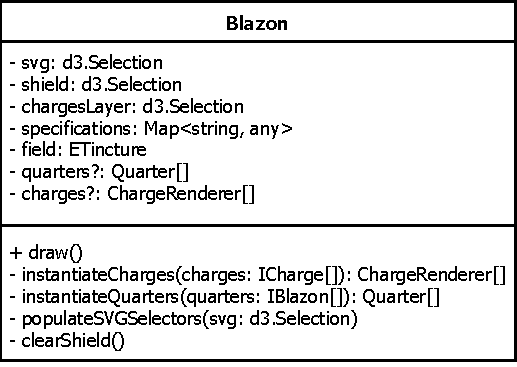
\includegraphics[width=0.5\linewidth]{BlazonUML}
  \caption{\texttt{Blazon} UML.}%
  \label{fig:BlazonUML}
\end{figure*}

\begin{figure*}[h]
  %\centering
  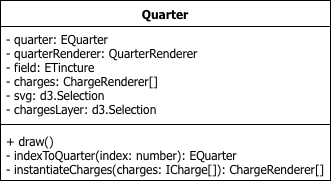
\includegraphics[width=0.5\linewidth]{QuarterUML}
  \caption{\texttt{Quarter} UML.}%
  \label{fig:QuarterUML}
\end{figure*}

\begin{figure*}[h]
  %\centering
  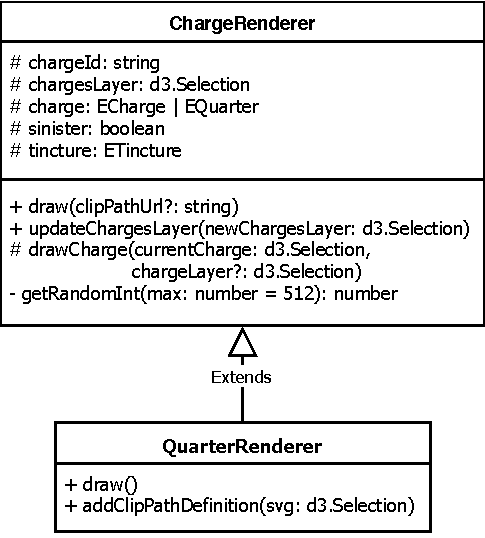
\includegraphics[width=0.5\linewidth]{ChargeRendererUML}%
  \caption{\texttt{ChargeRenderer} hierarchy and methods.}%
  \label{fig:charge_renderer_hierarchy}
\end{figure*}

\pagebreak%

\section{Third Design Iteration Diagrams}%
\label{sec:third_design_iteration_diagrams}

\begin{figure*}[h]
  %\centering
  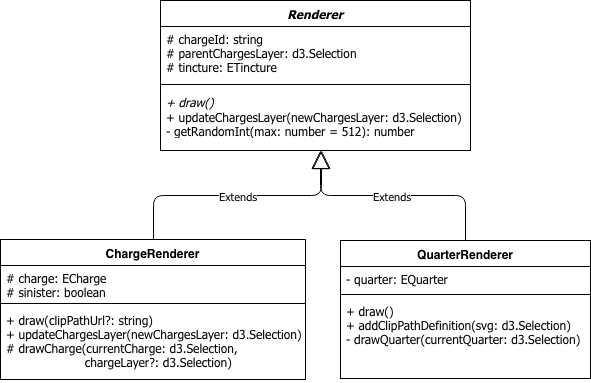
\includegraphics[width=0.8\linewidth]{RendererUML}
  \caption{\texttt{Renderer} hierarchy and methods.}%
  \label{fig:RendererUML}
\end{figure*}

\begin{figure*}[h]
  %\centering
  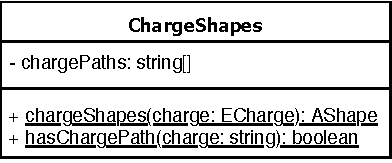
\includegraphics[width=0.5\linewidth]{ChargeShapesUML}
  \caption{\texttt{ChargeShapes} UML.}%
  \label{fig:ChargeShapesUML}
\end{figure*}

\begin{figure*}[h]
  %\centering
  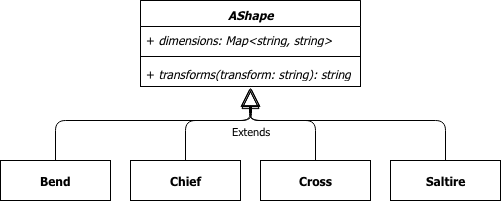
\includegraphics[width=0.8\linewidth]{AShapeUML}
  \caption{\texttt{AShape} hierarchy and methods.}%
  \label{fig:AShapeUML}
\end{figure*}

\setboolean{@mainmatter}{false}


\end{document}
